\documentclass[10pt,xcolor={table,dvipsnames}]{beamer} 		% carica automaticamente amsthm, amssymb, amsmath, graphicx

\usepackage[T1]{fontenc}				% codifica dei font
\usepackage[utf8]{inputenc}				% lettere accentate da tastiera
\usepackage[italian]{babel}				% lingua del documento
\usepackage[italian]{varioref}			% Per usare il comando \vref{label}, che dà dei collegamenti più dettagliati

% Load the custom style file
\usepackage{AndreaStyle}
% The file `AndreaStyle.sty` is stored in: `D:\Programmi e Applicazioni\texlive\texmf-local\tex\latex\local` for Windows.
% The file `AndreaStyle.sty` is stored in: `/usr/local/texlive/texmf-local/tex/latex/local` for Ubuntu (desktop).
% This won't work in Overleaf, until the AndreaStyle.sty file is added to the project

\usepackage{mathdots}

\usepackage{mathrsfs}					% Per dei caratteri matematici migliori: \mathscr{} e \mathcal{}
%\usepackage{braket} 					% Per il comando \Set, e altre (poche) cose
%\usepackage{textcomp}					% Dovrebbe aggiungere più simboli
\usepackage{bbm}						% Più simboli in \mathbb

%\usepackage{arydshln}					% per le linee tratteggiate nelle tabelle

%\usepackage[rightcaption]{sidecap}		% Per mettere le didascalie di lato

\usepackage{fontawesome5}				% Aggiunge simboli da FontAwesome

\usepackage{hyperref}					% Importante: hyperref va caricato nel documento.


%\setcounter{tocdepth}{1}	% profondità dell'indice

	% TEOREMI CUSTOM:
\theoremstyle{plain}					% Definisce ambienti per Teoremi, esercizi, corollari... Con lo stile adeguato
	\newtheorem{proposizione}{Proposizione}[section]
	\newtheorem*{proposizione*}{Proposizione}
	
	\newtheorem{teorema}{Teorema}[section]
	\newtheorem*{teorema*}{Teorema}
		
	%\newtheorem{lemma_es}{Lemma}[esercizio]
	%\newtheorem{lemma}{Lemma}[section]
	\newtheorem*{lemma*}{Lemma}
	\newtheorem{corollario}{Corollario}[section]


\theoremstyle{definition}				
	\newtheorem{definizione}{Definizione}[section]%[chapter]
	\newtheorem*{definizione*}{Definizione}	%definizione non numerata
	\newtheorem*{notazione}{Notazione}

\theoremstyle{remark}
	\newtheorem{oss}{Osservazione}[section]
	\newtheorem*{oss*}{Osservazione}


	% COMANDI CUSTOM
% Define the \indicator command
\NewDocumentCommand{\indicator}{O{t} O{m} O{i}}{%
  \mathlarger{\mathbbm{1}}\qty{\scriptstyle {x}_{#1}^{(#2)}=#3}%
}
% Define the \transpose command
\newcommand{\transpose}[1]{\prescript{t}{}{#1}}

	%COLORI
\definecolor{madridlightblue}{RGB}{233, 233, 243}
	

	
% ------------------------- INIZIO CODICE -------------------------
\usetheme{Madrid}


\title[Seminario MNCM]{Consistently Estimating Markov Chains with Noisy Aggregate Data}			%WIP
%\subtitle{Presentazione e dimostrazione della convergenza} 
\author{Andrea Marino}
\institute[DI UniPi]{Università di Pisa}
%\titlegraphic{\includegraphics[width=2cm]{Immagini/cherubino_black.eps}}
\date[\today]{Metodi Numerici per le Catene di Markov\newline Seminario di fine corso}

\AtBeginSection[] 						
{
	\begin{frame}
		\frametitle{Sommario}
		\tableofcontents[currentsection,subsectionstyle=show/show/hide] 
	\end{frame}
}

\begin{document}
	\begin{frame}[plain]
		\titlepage
	\end{frame}
	
\section*{Sommario}
	\setcounter{tocdepth}{1}
	\begin{frame}
		\frametitle{Sommario}
		\tableofcontents
	\end{frame}
	
	\setcounter{tocdepth}{2}

\section{Introduzione, notazione e prime definizioni}

	\begin{frame}{Introduzione al problema, notazione}%{Descrizione del contesto}
		Supponiamo di avere una popolazione di $N\in\mathbb{N}_{>0}$ individui che evolvono da 
		uno stato all'altro {\smaller ($S\in\mathbb{N}_{>0}$: numero di possibili stati)}, 
		\emph{indipendentemente}, per $T\in\mathbb{N}_{>0}$ istanti temporali 
		{\smaller ($[k]\coloneqq\qty{1,\dots,k}$)}:
		\[
			\qty{x_{t}^{(m)}}_{t\in[T]}\sim\mathrm{Markov}\qty(\pi_0,P)\qquad\forall\,m\in[N].
		\]
		%\vspace*{-\baselineskip}
		%\begin{itemize}
		%	%\item<2-> $N$: dimensione della popolazione, $T$: istanti temporali {\smaller(sarà $T\to\infty$)}
		%	\item<2-> $S\in\mathbb{N}_{>0}$: numero di possibili stati
		%	\item<3-> $P\in\R{S}{S}$: matrice di transizione, $\pi_0\in\R{S}$: distribuzione iniziale
		%\end{itemize}
		%\onslide<2->{$S\in\mathbb{N}_{>0}$: numero di possibili stati, 
		%$P\in\R{S}{S}$: matrice di transizione, 
		%$\pi_0\in\R{S}$: distribuzione iniziale,
		%$\pi\in\R{S}$: distribuzione invariante.}
		%\smallskip 
		
		\onslide<2->{Supponiamo inoltre che:}
		\begin{itemize}
			\item<2-> La catena sia \emph{ergodica} e omogenea nel tempo
			(cfr. Appendice~\hyperlink{frame:catena_ergodica:appendice}{\faHandPointRight}).

			$\pi\in\R{S}$: distribuzione invariante 
			\item<3-> $x_t^{(m)}$ non sia osservabile per alcun $t\in[T], m\in[N]$, 
			ma che vi sia una \emph{conta aggregata} $\vb*{n}_t\in\R{S}$, definita t.c.
			\vspace*{-0.5\baselineskip}
			\[
				\vb*{n}_t(i)\coloneqq\sum_{m=1}^N\indicator
			\]
			\vspace*{-0.9\baselineskip}
			%$\vb*{n}_t(i)\coloneqq\sum_{m=1}^N\indicator$
			\item<4-> I dati osservati siano $\qty{\vb*{y}_1,\dots,\vb*{y}_T}$, 
			$\vb*{y}_t$ è ottenuto 
			da $\vb*{n}_t$ tramite un modello del rumore $\P{\vb*{y}_t}{\vb*{n}_t}$
			\item<5-> La raccolta è ripetuta $K$ volte, restituendo 
			$\qty{\vb*{y}_1^{(k)},\dots,\vb*{y}_T^{(k)}}_{k\in[K]}$
		\end{itemize}
	\end{frame}

	\begin{frame}{Modello}
		\begin{figure}[ht]
			\centering
			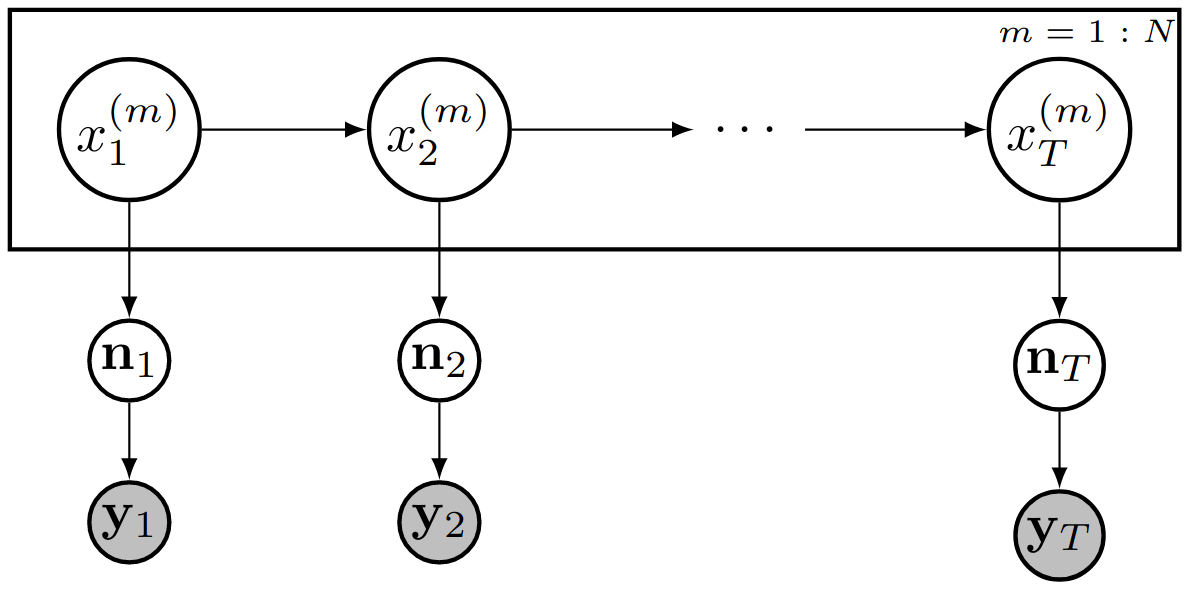
\includegraphics[width=0.45\textwidth]{Immagini/plate_model.png}
			\caption{\emph{Rappresentazione del modello in plate notation}}
		\end{figure}

		\vspace*{-0.5\baselineskip}
		La plate notation rappresenta graficamente come fattorizzare la legge congiunta:
		\begin{itemize}
			\item Cerchio vuoto: v.a. non osservata. Cerchio pieno: v.a. osservata
			\item<2-> Freccia: la v.a. in coda d'arco "influenza" la v.a. in testa
			\item<3-> Rettangolo: copia il contenuto tante volte quanto specificato dall'indice
		\end{itemize}

		%RIMANEGGIARE
		\begin{alertblock}<4->{Obiettivo}
			Usando le osservazioni
			$\big\{\vb*{y}_1^{(k)},\dots,\vb*{y}_T^{(k)}\big\}_{k\in [K]}$, stimare $P$.

			In particolare, vedremo come stimare $P$ usando il \emph{metodo dei momenti}.
			Lo stimatore dei momenti è consistente. 
		\end{alertblock}

	\end{frame}

	\begin{frame}
		{\hypertarget{frame:dettagli_nt}{Notazione, definizioni preliminari 3/3}}
		% Cura sottotitolo!
		%{Dettagli su $\vb*{n}_t$}
		\begin{definizione}
			Siano $\vb*{\mu}_t\in\R{S}$ e $\vb*{\mu}_{t,t+1}\in\R{S}{S}$ il vettore e la matrice
			delle leggi marginali:
			\vspace*{-0.5\baselineskip}
			\[\begin{aligned}
				\vb*{\mu}_t(i)=\P{x_t=i}=\qty(\transpose{\pi_0}P^t)_i & \qquad & \vb*{\mu}_{t,t+1}(i,j)=\P{x_t=i,x_{t+1}=j}\\
			\end{aligned}\]
		\end{definizione}

		\begin{oss}
			\begin{itemize}
				\item $\vb*{n}_t(i)=\sum_{m=1}^N\indicator$: numero di individui nello stato $i\in S$,
				al tempo $t\in T$.
				\item $\P{\indicator =1}=\P{x_t^{(m)}=i}=\vb*{\mu}_t(i)$
				\item $\vb*{n}_t$ è multinomiale di parametri $N,\vb*{\mu}_t$
				(cfr. Appendice~\hyperlink{frame:dettagli_nt:appendice}{\faHandPointRight})
			\end{itemize}
		\end{oss}

		\begin{oss}
			Si ha $P=\operatorname{Diag}\qty(\vb*{\mu}_t)^{-1}\cdot\vb*{\mu}_{t,t+1}$.

			Se $\pi_0=\pi$, $\vb*{\mu}_t=\pi\quad\forall\,t\in[T]$ e dunque 
			$\operatorname{Diag}\qty(\vb*{\mu}_t)$ è invertibile. 
			Altrimenti, $\vb*{\mu}_t>0$ per $t$ grande abbastanza. 
			%infatti 
			%$P_{i,j}=\P{x_{t+1}=j}{x_t=i}=\P{x_t=i,x_{t+1}=j}/\,\P{x_t=i}=\vb*{\mu}_{t,t+1}(i,j)/\,\vb*{\mu}_t(i)$
		\end{oss}


	\end{frame}











	

    
\section{Ringraziamenti e bibliografia}
    \begin{frame}
        \begin{center}
            \Huge{Grazie per l'attenzione!}
        \end{center}
    \end{frame}

	\begin{frame}{\refname}
		\begin{thebibliography}{9}
			\bibitem{article:main} Garrett Bernstein, Daniel Sheldon
			\newblock Consistently Estimating Markov Chains with Noisy Aggregate Data
			\newblock Proceedings of the 19th International Conference on Artificial Intelligence and Statistics, \emph{PMLR}, vol. 51, pp. 1142-1150, PMLR (2016) 09-11 May

		\end{thebibliography}
	\end{frame}

\section*{Appendice}
	\begin{frame}
		\begin{center}
			\Huge{\textbf{Appendice}}
		\end{center}
	\end{frame}

	\begin{frame}
		{\hypertarget{frame:catena_ergodica:appendice}{Catene di Markov ergodiche}}
		\begin{definizione}
			Ricordiamo che una catena di Markov è detta \alert{ergodica} se è
			irriducibile, positiva ricorrente e aperiodica.
		\end{definizione}
		\onslide<2->{Una catena ergodica {\smaller (in quanto irriducibile e positiva 
		ricorrente)} ha una distribuzione invariante $\pi$. Inoltre:}
		\begin{itemize}
			\item<2-> $\pi$ è unica
			\item<3-> $\pi_i=1/\,\mathbb{E}_i\qty[T_i]$ 
			{\smaller (ovvero 1/tempo atteso di ritorno)}, dove 
			$T_i\coloneqq\inf_{n\ge 1}\qty{X_n=i}$ {\smaller (istante di primo passaggio)},
			e in particolare $\pi_i>0$			
		\end{itemize}
		\begin{oss}<4->
			Per una catena finita e irriducibile {\smaller (dunque positiva ricorrente)},
			le due condizioni precedenti si possono ricavare dal teorema di Perron-Frobenius.
		\end{oss}

		\onslide<5->{Il \emph{teorema di convergenza all'equilibrio} dice che per una 
		catena ergodica vale $\lim_{n\to\infty}\P{x_n=i}=\pi_i$. 
		In particolare $P_{i,j}\overset{n}{\longrightarrow}\pi_j\quad\forall\,i,j\in[S]$.}
		\vfill

		(Indietro:~\hyperlink{frame:intro}{\faHandPointLeft})
	\end{frame}

	\begin{frame}
		{\hypertarget{frame:dettagli_nt:appendice}{Dettagli sulla legge di $\vb*{n}_t$}}		
		$\R{S}\ni\vb*{n}_t$, e $\vb*{n}_t(i)=\sum_{m=1}^N\indicator$.
		\smallskip

		\onslide<2->{Possiamo interpretare $\vb*{n}_t$ come la somma di $N$ v.a. i.i.d.
		$V_t^{(1)},\dots,V_t^{(N)}$, ciascuna delle quali codifica lo stato 
		dell'individuo $m\in[N]$ corrispondente, al tempo $t\in[T]$.}

		\onslide<3->{$V_t^{(m)}$ rappresenta il risultato di una "prova" con $S$ 
		possibili \emph{outcomes}. L'outcome $i\in [S]$ è rappresentato dal versore 
		canonico $e_i\in\R{S}$.} 
		\onslide<4->{Si ha: 
		\[
			\P{V_t^{(m)}=e_i}=\P{x_t^{(m)}=i}=\vb*{\mu}_t(i)
		\]
		dunque $V_t^{(m)}$ è \emph{categorica} di parametro $\vb*{\mu}_t$, 
		$\forall\,m\in[N]$.} 
		\onslide<5->{Di conseguenza $\vb*{n}_t$ è multinomiale di 
		parametri $N,\vb*{\mu}_t$.}
		\bigskip 

		\textcolor{red}{Disegno}
		\vfill
		
		(Indietro:~\hyperlink{frame:dettagli_nt}{\faHandPointLeft})
	\end{frame}




\end{document}

